\documentclass{beamer}

\usepackage{préambule}
\usepackage{tkz-tab}

\setbeamersize{
	text margin left=0.5cm,
	text margin right=0.5cm
}
\setlength{\columnseprule}{0.7pt}

\begin{document}
\small

\begin{frame}
	\begin{multicols}{2}
		\begin{center}
			\begin{tikzpicture}[scale=0.5]
				\draw[thin,gray] (-3.5,-2.5) grid (5.5,6.5);
				\draw[thick,\myArrow] (-3.5,0) -- (5.5,0);
				\draw[thick,\myArrow] (0,-2.5) -- (0,6.5);
				\draw[thick] (1,0) -- ++(0,-0.2) node[below] {$1$};
				\draw[thick] (0,1) -- ++(-0.2,0) node[left] {$1$};

				\draw[very thick,violet,variable=\x,domain=-3:5] plot({\x},{-1/2*\x + 1}) node[right] {$𝒞_f$};
				\draw[very thick,orange,variable=\x,domain=-3:5] plot({\x},{(\x*\x - 2*\x - 3) / 2})  node[right] {$𝒞_g$};
			\end{tikzpicture}
		\end{center}

		\begin{enumerate}
			\item Donner les tableaux de signes des fonctions $f$ et $g$ ci-dessus.
			\item Donner les tableaux de variations des fonctions $f$ et $g$ ci-dessus.
			\item Soit $h$ la fonction telle que $h(x) = -x² + 3$. Calculer en détaillant le taux de variation de $h$ entre $3$ et $5$. % (f(5) - f(3)) / (5 - 3) = (-25 + 3 + 9 - 3) / 2 = -16/2 = -8
		\end{enumerate}

		\columnbreak

		\begin{center}
			\begin{tikzpicture}[scale=0.5]
				\draw[thin,gray] (-3.5,-6.5) grid (5.5,2.5);
				\draw[thick,\myArrow] (-3.5,0) -- (5.5,0);
				\draw[thick,\myArrow] (0,-6.5) -- (0,2.5);
				\draw[thick] (1,0) -- ++(0,-0.2) node[below] {$1$};
				\draw[thick] (0,1) -- ++(-0.2,0) node[left] {$1$};

				\draw[very thick,violet,variable=\x,domain=-3:5] plot({\x},{2/3*\x - 2}) node[right] {$𝒞_f$};
				\draw[very thick,orange,variable=\x,domain=-3:5] plot({\x},{(-\x*\x + 2*\x + 3) / 2})  node[right] {$𝒞_g$};
			\end{tikzpicture}
		\end{center}

		\begin{enumerate}
			\item Donner les tableaux de signes des fonctions $f$ et $g$ ci-dessus.
			\item Donner les tableaux de variations des fonctions $f$ et $g$ ci-dessus.
			\item Soit $h$ la fonction telle que $h(x) = x² - 2x$. Calculer en détaillant le taux de variation de $h$ entre $3$ et $5$. % (f(5) - f(3)) / (5 - 3) = (25 - 10 - 9 + 6) / 2 = 12 / 2 = 6
		\end{enumerate}
	\end{multicols}
\end{frame}

\begin{frame}
	\uline{Correction sujet de gauche (A) :}

	\begin{enumerate}
		\item 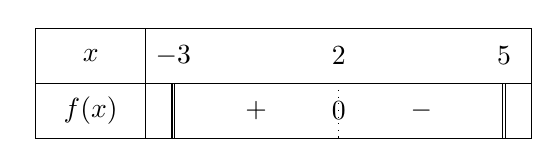
\begin{tikzpicture}[scale=0.7]
			      \tkzTabInit{$x$ / 1 , $f(x)$ / 1}{$-3$, $2$, $5$}
			      \tkzTabLine{d, +, z, -, d}
		      \end{tikzpicture}

		      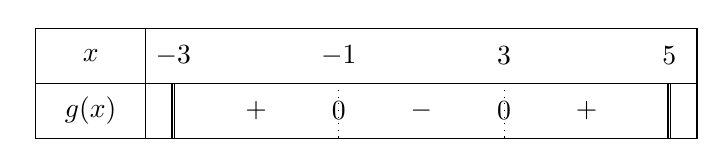
\begin{tikzpicture}[scale=0.7]
			      \tkzTabInit{$x$ / 1 , $g(x)$ / 1}{$-3$, $-1$, $3$, $5$}
			      \tkzTabLine{d, +, z, -, z, +, d}
		      \end{tikzpicture}
		\item 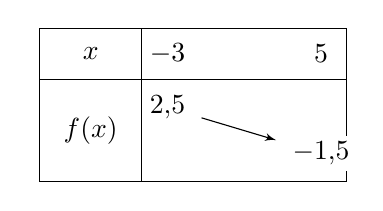
\begin{tikzpicture}[scale=0.65]
			      \tkzTabInit{$x$ / 1 , $f(x)$ / 2}{$-3$, $5$}
			      \tkzTabVar{+/ $2{,}5$, -/ $-1{,}5$}
		      \end{tikzpicture}
		      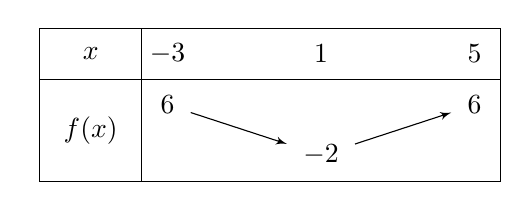
\begin{tikzpicture}[scale=0.65]
			      \tkzTabInit{$x$ / 1 , $f(x)$ / 2}{$-3$, $1$, $5$}
			      \tkzTabVar{+/ $6$, -/ $-2$, +/ $6$}
		      \end{tikzpicture}
		\item $\dfrac{h(5) - h(3)}{5 - 3} = \dfrac{(-5² + 3) - (-3² + 3)}{2} = \dfrac{-22 - (-6)}{2} = \dfrac{-16}{2} = -8$
	\end{enumerate}
\end{frame}

\begin{frame}
	\uline{Correction sujet de droite (B) :}

	\begin{enumerate}
		\item 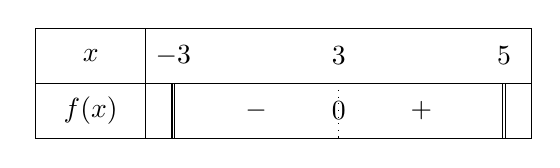
\begin{tikzpicture}[scale=0.7]
			      \tkzTabInit{$x$ / 1 , $f(x)$ / 1}{$-3$, $3$, $5$}
			      \tkzTabLine{d, -, z, +, d}
		      \end{tikzpicture}

		      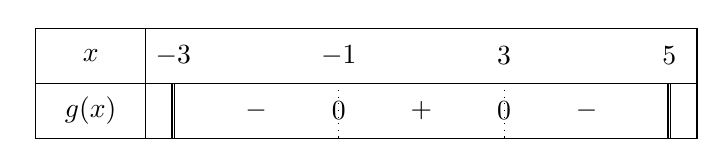
\begin{tikzpicture}[scale=0.7]
			      \tkzTabInit{$x$ / 1 , $g(x)$ / 1}{$-3$, $-1$, $3$, $5$}
			      \tkzTabLine{d, -, z, +, z, -, d}
		      \end{tikzpicture}
		\item 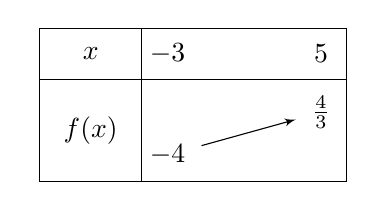
\begin{tikzpicture}[scale=0.65]
			      \tkzTabInit{$x$ / 1 , $f(x)$ / 2}{$-3$, $5$}
			      \tkzTabVar{-/ $-4$, +/ $\frac{4}{3}$}
		      \end{tikzpicture}
		      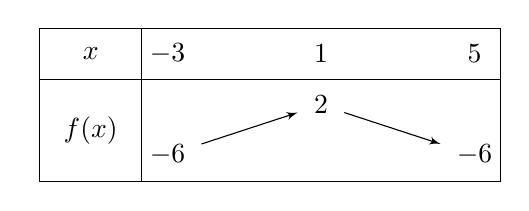
\begin{tikzpicture}[scale=0.65]
			      \tkzTabInit{$x$ / 1 , $f(x)$ / 2}{$-3$, $1$, $5$}
			      \tkzTabVar{-/ $-6$, +/ $2$, -/ $-6$}
		      \end{tikzpicture}
		\item $\dfrac{h(5) - h(3)}{5 - 3} = \dfrac{(5² - 2×5) - (3² - 2×3)}{2} = \dfrac{15 - 3}{2} = \dfrac{12}{2} = 6$
	\end{enumerate}
\end{frame}

\end{document}